% SPDX-FileCopyrightText: 2023 SAP SE
%
% SPDX-License-Identifier: Apache-2.0
%
% This file is part of FEDEM - https://openfedem.org

%%%%%%%%%%%%%%%%%%%%%%%%%%%%%%%%%%%%%%%%%%%%%%%%%%%%%%%%%%%%%%%%%%%%%%%%%%%%%%%%
%
% FEDEM Theory Guide.
%
%%%%%%%%%%%%%%%%%%%%%%%%%%%%%%%%%%%%%%%%%%%%%%%%%%%%%%%%%%%%%%%%%%%%%%%%%%%%%%%%

\chapter{Simulation Results}

\iftoggle{publicedition}{}{% The following is for the in-house edition only.

\section{Primary simulation variables}

The primary simulation variables are the supernode orientation and position,
the supernode translational and rotational velocity and acceleration,
and the current superelement transformation matrix.
Variables from the control simulation (the control variables), and the joint
variables are also primary variables in the simulation.

The orientation and position of the supernodes are represented as a $(3\times4)$
transformation matrix (see \eqsref{eq:posDef}{eqSC:Png}):
%
\begin{equation}
{\mf P}_{NG} \;=\; \left[ \begin{array}{*{20}c}
R_{11} & R_{12} & R_{13} & p_x \\
R_{21} & R_{22} & R_{23} & p_y \\
R_{31} & R_{32} & R_{33} & p_z \\
\end{array} \right] \;=\; \left[ \begin{array}{cccc}
{\mf i}_x & {\mf i}_y & {\mf i}_z & {\mf p}
\end{array}\right]
\label{eqK43:1}
\end{equation}
%
where ${\mf i}_x$, ${\mf i}_y$, and ${\mf i}_z$ are unit vectors in the $x$-,
$y$-, and $z$-directions, respectively, of the supernode coordinate system, and
the vector ${\mf p}$ represents the position of supernodes, all of which are
referred to in the global coordinate system.
The three unit vectors represent the direction cosine matrix, which uniquely
defines the orientation in space.

The supernode velocities are presented by two Cartesian vectors, one of which
represents the translational velocity, and one the rotational velocity relative
to the global coordinate system as shown below:
%
\begin{equation}
\left[\begin{array}{c} {\mf v_t} \\ {\mf v_r} \end{array}\right] \;=\;
\left[\begin{array}{cccccc}
v_{tx} & v_{ty} & v_{tz} & v_{rx} & v_{ry} & v_{rz}
\end{array}\right]^T
\label{eqK43:2}
\end{equation}
%
where
%
\begin{namelist}{$\quad{\mf v_r}$}
\item[$\quad{\mf v_t}$] represents the translational velocity vector, and
\item[$\quad{\mf v_r}$] represents the rotational velocity vector
(angular velocity).
\end{namelist}

The supernode accelerations are similarly presented as two Cartesian vectors
relative to the global coordinate system as shown below:
%
\begin{equation}
\left[\begin{array}{c} {\mf a_t} \\ {\mf a_r} \end{array}\right] \;=\;
\left[\begin{array}{cccccc}
a_{tx} & a_{ty} & a_{tz} & a_{rx} & a_{ry} & a_{rz}
\end{array}\right]^T
\label{eqK43:3}
\end{equation}
%
where
%
\begin{namelist}{$\quad{\mf a_r}$}
\item[$\quad{\mf a_t}$] represents the translational acceleration vector, and
\item[$\quad{\mf a_r}$] represents the rotational acceleration vector
(angular acceleration).
\end{namelist}

The magnitudes for the modal supernode displacement, velocity, and acceleration,
which represent fixed interface superelement modes of vibration
(described in Section~\ref{secCMS:FixeIntMode}), are presented in a similar way
to that of ordinary supernodes, with the exception that there are a variable
number of DOFs per supernode.
The variables for a modal supernode may be written:
%
\begin{equation}
\left[\begin{array}{ccc}
{\mf y} & \dot{\mf y} & \ddot{\mf y} \end{array}\right] \;=\;
\left[ \begin{array}{*{20}c}
y_1 & \dot{y}_1 & \ddot{y}_1 \\
y_2 & \dot{y}_2 & \ddot{y}_2 \\
\vdots & \vdots & \vdots \\
y_n & \dot{y}_n & \ddot{y}_n
\end{array} \right]
\label{eqK43:4}
\end{equation}
%
where
%
\begin{namelist}{$\quad\ddot{\mf y}$}
\item[$\quad{\mf y}$]      is the modal supernode displacement magnitude,
\item[$\quad\dot{\mf y}$]  is the modal supernode velocity magnitude, and
\item[$\quad\ddot{\mf y}$] is the modal supernode acceleration magnitude.
\end{namelist}

The superelement position and orientation are represented as a $(3\times4)$
transformation matrix (see \eqsref{eq:posDef}{eqK43:1}):
%
\begin{equation}
{\mf P}_{SG} \;=\; \left[ \begin{array}{*{20}c}
R_{11} & R_{12} & R_{13} & o_x \\
R_{21} & R_{22} & R_{23} & o_y \\
R_{31} & R_{32} & R_{33} & o_z \\
\end{array} \right] \;=\; \left[\begin{array}{cccc}
{\mf i}_x & {\mf i}_y & {\mf i}_z & {\mf o} \end{array}\right]
\label{eqK43:5}\end{equation}
%
where the unit vectors ${\mf i_x}$, ${\mf i_y}$ and ${\mf i_z}$ represent the
orientation of the superelement coordinate system, while ${\mf o}$ represents
the origin's position in the superelement coordinate system.

As previously stated, control variables are also primary simulation variables.
The control variables are defined as input, state, and algebraic variables.

\section{Derived simulation variables}

The following simulation variables are derived from the primary variables:
%
\begin{itemize}
\item   Spring variables
\item   Damper variables
\item   Forces and torques
\end{itemize}

A spring element is a uniaxial or a joint spring and has three variables:
The spring length/angle; the spring deflection from the stress-free position;
and the spring force/torque.
The spring length of a uniaxial spring is calculated from the position of the
two end nodes.
In case of joint springs, the spring length or angle refers to a joint variable.
Subtracting the specified stress-free length/angle of the spring from the
calculated length/angle of the spring gives the spring deflection.
In the general nonlinear case, the spring force/torque is found by integrating
the spring stiffness over the spring deflection.

A damper element is a uniaxial or joint damper and has three variables:
The damper length/angle; the damper relative velocity;
and the damper force/torque.
The damper length of uniaxial dampers is calculated from the position of
the two end nodes.
In case of joint dampers, the damper length or angle refers to a joint variable.
Damper velocity for uniaxial dampers is calculated from the end node velocities.
Denoting the global coordinates of the two end points of the damper as
%
\begin{equation}
{\mf p}_1 \;=\;
\left[ \begin{array}{*{20}c} x_1 \\ y_1 \\ z_1 \end{array} \right]
\quad\text{and}\quad
{\mf p}_2 \;=\;
\left[ \begin{array}{*{20}c} x_2 \\ y_2 \\ z_2 \end{array} \right]
\label{eqK43:6}
\end{equation}
%
the damper unit direction vector is calculated from
%
\begin{equation}
{\mf e}_{12} \;=\; \frac{{\mf p}_2 - {\mf p}_1}{\|{\mf p}_2 - {\mf p}_1\|}
\label{eqK43:7}
\end{equation}
%
The relative velocity for these two points may be calculated from
%
\begin{equation}
{\mf v}_{12} \;=\;
\left[ \begin{array}{*{20}c}
\dot{x}_1 \\ \dot{y}_1 \\ \dot{z}_1
\end{array} \right] -
\left[ \begin{array}{*{20}c}
\dot{x}_2 \\ \dot{y}_2 \\ \dot{z}_2
\end{array} \right]
\label{eqK43:8}
\end{equation}
%
and the damper velocity is then calculated from the scalar product
%
\begin{equation}
{\mf v}_D \;=\; {\mf e}_{12}^T {\mf v}_{12}
\label{eqK43:9}
\end{equation}
%
In the case of joint dampers, the damper velocity refers directly to a joint
variable velocity.
The damper force/torque is found by multiplying the damping coefficient by the
damper velocity.

For calculation of superelement node forces and torques, refer to the stiffness
relation of \eqnref{eqSC:forceLocal}, see Section~\ref{sec:SupElIntForce}.
The forces are transformed to global direction and added into the system vector.
This system vector is then used to present the nodal forces and torques in
relation to a global coordinate system.
Joint forces and torques are found on the corresponding master or slave DOFs
of the joint, and based on the superelement forces from deformation,
\eqnref{eqSC:forceLocal}, combined with the contributions from inertia
and damping, we get:
%
\begin{equation}
\tilde{\mf f}_e \;=\;
\tilde{\mf k}_e \tilde{\mf v}_d +
\tilde{\mf c}_e \dot{\tilde{\mf v}} +
\tilde{\mf m}_e \ddot{\tilde{\mf v}}
\label{eqSR:TotalSupElForce}
\end{equation}

\section{Substructure retracking}

The co-rotated superelement formulation developed in
Chapter~\ref{chap:SupElCorot} shows the derivation of the superelement
deformation vector for an external node, \eqnref{eqSC:nodeDefDisp}.
The modal coordinates ${\mf y}$ are primary integration variables;
and the superelement deformation vectors for all external nodes and modal
coordinates are given by \eqnref{eqSC:supelDefDisp}.

The inverse CMS transformation gives
%
\begin{equation}
\label{eqK43:10}
\eqalign{
{\mf v}_i \;=\; & {\mf v}_i^i + {\mf v}_i^e \cr
            =\; & {\mf B} {\mf v}_e + {\tf \Phi}{\mf y}
}
\end{equation}
%
and the expanded substructure displacement vector may be written
%
\begin{equation}
{\mf v} \;=\;
\left[ \begin{array}{c} {\mf v}_e \\ {\mf v}_i \end{array} \right] \;=\;
{\mf H} \left[ \begin{array}{c} {\mf v}_e \\ {\mf y} \end{array} \right]
\label{eqK43:11}
\end{equation}
%
(see \eqnref{eqCMS:Hdef}).

Nodal displacements for substructure primary element $j$ may now be extracted
from the substructure displacement vector:
%
\begin{equation}
{\mf u}_j \;=\; {\mf A}_j {\mf v}
\label{eqK43:13}
\end{equation}
%
where
%
\begin{namelist}{${\mf u}_j$}
\item[${\mf u}_j$] represents the displacement vector of primary element $j$
in the substructure,
\item[${\mf A}_j$] is the incidence matrix that represents the topology
for primary element $j$ in the substructure, and
\item[${\mf v}$] is the substructure displacement vector of \eqnref{eqK43:10}.
\end{namelist}

\section{Finite element stress analysis}

The strain field within a finite element is expressed by the nodal DOFs
${\mf u}$ and a set of interpolation polynomials.
For instance, for a membrane finite element:
%
\begin{equation}
{\mf\varepsilon}(x,y) \;=\; \bar{\mf B}(x,y)\,{\mf u}
\label{eqK43:17}
\end{equation}
%
where
%
\begin{namelist}{$\quad\bar{\mf B}$}
\item[$\quad{\tf\varepsilon}$] is the element strain vector, and
\item[$\quad\bar{\mf B}$]      is the strain interpolation matrix,
\end{namelist}
%
The stress is then according to Hooke's Law:
%
\begin{equation}
{\tf\sigma} \;=\; {\mf C} {\tf\varepsilon}
\label{eqK43:18}
\end{equation}
%
where
%
\begin{namelist}{$\quad{\mf E}$}
\item[$\quad{\tf\sigma}$] is the element stress vector, and
\item[$\quad{\mf C}$] is the constitutive matrix.
\end{namelist}
%
For further details, refer to textbooks on the finite element method.

% SPDX-FileCopyrightText: 2023 SAP SE
%
% SPDX-License-Identifier: Apache-2.0
%
% This file is part of FEDEM - https://openfedem.org

%%%%%%%%%%%%%%%%%%%%%%%%%%%%%%%%%%%%%%%%%%%%%%%%%%%%%%%%%%%%%%%%%%%%%%%%%%%%%%%%
%
% FEDEM Theory Guide.
%
%%%%%%%%%%%%%%%%%%%%%%%%%%%%%%%%%%%%%%%%%%%%%%%%%%%%%%%%%%%%%%%%%%%%%%%%%%%%%%%%

\section{Virtual strain gauges}

The strains computed from a finite element provide the basis for computing the
strain-rosette strains.
Both three- and four-node strain-measuring elements can be defined,
with the strain computations at the centroid of both elements.
The membrane formulation of the elements is a constant strain triangle and a
bi-linear quadrilateral element with a $C^0$ bending approach.
The strains of these elements can be expressed as
%
\begin{equation}
\tilde{\tf\varepsilon} \;=\; \tilde{\mf B} \tilde{\mf v}
\end{equation}
%
where $\tilde{\mf B}$ is the strain-displacement matrix in the local element
coordinate system.

The strain-rosette element is defined by the user and overlaid on the
actual FE mesh.
It does not, however, contribute any stiffness to the structure.
It exists only as a post-processing device for the purpose of calculating
the strains at that location.

The Cartesian strains in the rosette coordinate system can be computed as
%
\begin{equation}
\eqalign{
{\tf\varepsilon}_r \;=\; {\mf T}_{\varepsilon_r} \tilde{\tf\varepsilon}
\quad \text{where} & \quad
{\mf T}_{\varepsilon_r} = \left[ \begin{array}{*{20}c}
c_{11}^2  & c_{12}^2 & c_{11} c_{12} \\
c_{21}^2  & c_{22}^2 & c_{21} c_{22} \\
2c_{11} c_{21} & 2c_{22} c_{12} & (c_{11} c_{22} + c_{12} c_{21})
\end{array} \right] \cr
\text{and} & \quad c_{ij} \;=\; {\tf i}_i^r \cdot {\tf i}_j
}
\end{equation}
%
where ${\tf i}_i^r$ are base vectors for the rosette coordinate system, and
${\tf i}_j$ are base vectors for the element coordinate system.

Once the Cartesian strains ${\tf \varepsilon}_r$ are established, the user can
compute the strain for each leg of the rosette ${\tf\varepsilon}_l$, defined by
the unit direction vector ${\tf i}^l$ of the leg
%
\begin{equation}
\eqalign{
{\varepsilon}_l \;=\; {\mf t}_l {\tf\varepsilon}_r \quad \text{where} & \quad
{\mf t}_l \;=\; \left[ \begin{array}{ccc}
c_{l1}^2 & c_{l2}^2 & c_{l1}\:c_{l2}
\end{array} \right] \cr
\text{and} & \quad c_{lj} = {\tf i}_l \cdot {\tf i}_j^r
}
\end{equation}

\subsection{Recovering the element displacement vectors}

To compute the element strains and the strain gauge readings,
the element displacement vector $\tilde{\mf v}$ must be recovered from the
superelement displacement vector ${\mf v}_s$.

The free (unconstrained) DOFs for a superelement can be recovered from the
external triad DOFs ${\mf v}_{se}$, and the external DOFs ${\mf y}$ can be
recovered by means of the inverse CMS-transformation of Chapter~\ref{chap:CMS},
(see \eqnref{eqCMS:Hdef}):
%
\begin{equation}
{\mf v}_{\text{free}} \;=\; {\mf H v}_s \quad\text{or}\quad
\left[\begin{array}{c} {\mf v}_i \\ {\mf v}_e \end{array}\right] \;=\;
\left[\begin{array}{cc} {\mf B} & {\tf\Phi} \\ {\mf I} & {\mf 0}
\end{array}\right]
\left[\begin{array}{c} {\mf v}_{se} \\ {\mf y}
\end{array}\right]
\end{equation}
%
The columns of matrix $\mf B$ are displacement vectors; these vectors represent
the static displacements that occur when each of the external triad DOFs is
subjected to a unit displacement, one at a time.
The eigenvectors of the superelement are contained by $\tf\Phi$ when all the
external triad DOFs are fixed.

In addition, the full set of DOFs has to be recovered from possible linear
couplings by means of the matrix relationship\footnote{\label{effNote}
Numerically, this is handled in a much more efficient manner.}
%
\begin{equation}
{\mf v}_\text{full} \;=\; {\mf L v}_\text{free}
\end{equation}
%
where it is assumed that no prescribed displacements are allowed on the
internal DOFs, i.e., prescribed displacements can exist on external DOFs only.

The element displacement vector can now be extracted from the full system
displacement vector as$^\text{\ref{effNote}}$
%
\begin{equation}
{\mf v} \;=\; {\mf A v}_\text{full}
\end{equation}
%
where $\mf A$ is the incidence matrix containing only $0$s and $1$s,
collecting the correct DOFs from the full superelement vector.

Transformation to the local element coordinate system is handled by
%
\begin{equation}
\eqalign{
\tilde{\mf v} \;=\; {\mf T v} \quad \text{where} & \quad
{\mf T} \;=\; \left\lceil\begin{array}{ccc}
{\mf t} & \cdots & {\mf t}
\end{array}\right\rfloor \cr \text{and} & \quad
{\mf t} \;=\; \left[\begin{array}{ccc}
{\tf i}_1\cdot{\tf I}_1 & {\tf i}_1\cdot{\tf I}_2 & {\tf i}_1\cdot{\tf I}_3 \\
{\tf i}_2\cdot{\tf I}_1 & {\tf i}_2\cdot{\tf I}_2 & {\tf i}_2\cdot{\tf I}_3 \\
{\tf i}_3\cdot{\tf I}_1 & {\tf i}_3\cdot{\tf I}_2 & {\tf i}_3\cdot{\tf I}_3
\end{array}\right]
}
\end{equation}
%
using $\lceil\;\rfloor$ to signify the diagonal matrix.

The superelement-to-element displacement relationship can now be written:

\begin{equation}
\tilde{\mf v} \;=\; {\mf E}{\mf v}_s
\quad\text{where}\quad
{\mf E} = {\mf T A L H}
\end{equation}

\subsection{Strain displacement relationship for the strain-rosette}

The strain displacement matrix for the Cartesian strains in the rosette
coordinate system can now be established at the element location as a function
of the superelement DOFs, expressed as:
%
\begin{equation}
\label{eq:rosette strain}
{\tf \varepsilon}_r = {\mf B}{\mf v}_s
\quad\text{where}\quad
{\mf B} \;=\; {\mf T}_{\varepsilon r} \tilde {\mf B E}
\end{equation}

\remark{The strain-displacement matrix ${\mf B}$ of \eqnref{eq:rosette strain}
is computed for each rosette during initialization and stored in memory while
computing the strains for a time series.
${\mf B} = {\mf T}_{\varepsilon r} \tilde{\mf B}{\mf E}$ is thus computed once,
whereas ${\varepsilon}_r = {\mf B}{\mf v}_s$ is computed for each time step.}

The strain-gauge readings for each leg are then obtained from the Cartesian
strains as
%
\begin{equation}
\label{eq:gage strain}
\varepsilon_l \;=\; {\mf t}_l {\tf\varepsilon}_r
\quad\text{and}\quad
\sigma_l \;=\; {\mf t}_l {\mf C} {\tf\varepsilon}_r
\end{equation}
%
where $\mf C$ is the constitutive matrix from \eqnref{eqK43:18}.

} % End in-house edition only
% SPDX-FileCopyrightText: 2023 SAP SE
%
% SPDX-License-Identifier: Apache-2.0
%
% This file is part of FEDEM - https://openfedem.org

%%%%%%%%%%%%%%%%%%%%%%%%%%%%%%%%%%%%%%%%%%%%%%%%%%%%%%%%%%%%%%%%%%%%%%%%%%%%%%%%
%
% FEDEM Theory Guide.
%
%%%%%%%%%%%%%%%%%%%%%%%%%%%%%%%%%%%%%%%%%%%%%%%%%%%%%%%%%%%%%%%%%%%%%%%%%%%%%%%%

\section{Fatigue analysis}

Through fatigue analysis, one can asses the estimated life of a structural
component subjected to cyclic or repetitive loads, based on the computed
stress or strain history and some additional material properties.

The input to the fatigue analysis is the stress/strain reading in a virtual
strain gauge for each time step of the dynamics simulation,
\iftoggle{publicedition}{% The following is for the public edition
or alternatively one can compute the
{\em Signed absolute max\/} principal strain from the strain rosette tensor.
}{% The following is for the in-house edition only
\eqnref{eq:gage strain}, or alternatively one can compute the
{\em Signed absolute max\/} principal strain from the strain rosette tensor
given by \eqnref{eq:rosette strain}.
}% End in-house edition only
Letting $\{\varepsilon_1,\varepsilon_2\}$ denote the maximum and minimum
principal strains\footnote{These quantities are the same as the largest and
smallest eigenvalues of the symmetric strain tensor.}, respectively, the
signed absolute max value is defined through
%
\begin{equation}
\label{eq:signed abs max}
\varepsilon_\text{samax} \;=\; \left\{ \varepsilon_i :
|\varepsilon_i| = \max\{|\varepsilon_1|,|\varepsilon_2|\} \right\}
\end{equation}
%
Similarly, one can derive the signed absolute max principal stress,
$\sigma_\text{samax}$ from the stress tensor.
Using \eqnref{eq:signed abs max} will normally give a more conservative life
assessment compared to using a gauge leg reading, in cases where direction of
the maximum strain varies during the simulated event.
Using a gauge strain directly does not account for such variations.

\subsection{Peak valley extraction}

The first step in the process of obtaining the estimated life at a given point,
is to simplify the stress/strain history curve measured by the virtual strain
gauge, and removing oscillations smaller than a given threshold (gate value).
This is a process often referred to as {\em peak valley extraction\/}.

Consider the typical stress history reading, i.e., $\sigma_\text{samax}(t)$,
in Figure~\ref{fig:PVX}a), which typically consists of hundreds
(if not thousands) of data points.
In a life assessment, it is only the turning points of the curve that matter,
i.e., where the gradient of the curve changes sign.
Thus, after peak valley extraction using a gate value of 1 MPa,
the processed curve ends up as shown in Figure~\ref{fig:PVX}b).
The number of data points has been reduced from 201 to only 22 in this case.

\begin{figure}[b]
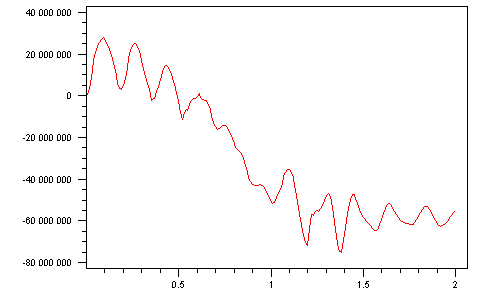
\includegraphics[width=0.5\textwidth]{Figures/LoaderRos9_sigma.png}
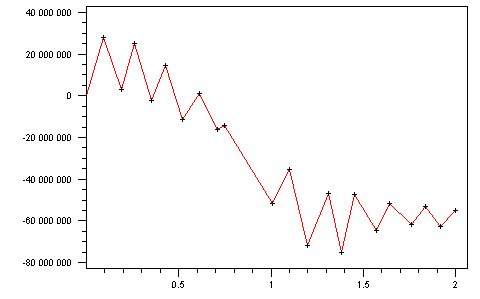
\includegraphics[width=0.5\textwidth]{Figures/LoaderRos9_pvx.png}
a) \hskip 0.5\textwidth b)
\caption{Peak valley extraction of a stress history curve.
a) The original stress curve.
b) The processed curve consisting of the turning points (+) only.}
\label{fig:PVX}
\end{figure}

\subsection{Rainflow analysis}

The next step of the fatigue analysis is to perform a {\em rainflow counting\/}
on the processed stress/strain signal, in order to further reduce a spectrum of
varying stresses/strains into a set of simple stress/strain reversals.
The process is named rainflow counting because it can be explained by viewing
the stress history curve like the one in Figure~\ref{fig:PVX}b) as a series of
Padoga roofs when it is rotated 90 degrees with the time axis vertically,
and letting drops of water flow from each peak and valley.
The stress cycles are then defined by how each flow of water is terminated
according to a set of rules.

In the algorithm adopted in Fedem, we traverse the peak and valley curve in
steps looking at three line segments defined by four neighboring points of the
curve (labeled 1, 2, 3, 4) in each step:
If the middle line 2-3 is shorter than both end lines 1-2 and 3-4, and its
gradient has opposite sign as the gradient of both lines 1-2 and 3-4, then
the points 2 and 3 define a full stress cycle and is removed from the curve.
We then proceed to the next step in which the previous point 4 becomes the
new point 2, while the subsequent two points in the curve become the new points
3 and 4.
If the points 2 and 3 were not removed, all four point counters are incremented
while proceeding to the next step.
We then continue until the entire curve has been traversed once.

The traversal is then restarted from the beginning of the curve, and
repeated until no more full cycles could be found during one traversal.
This process is illustrated in Figure~\ref{fig:Rainflow1} for the stress
curve of Figure~\ref{fig:PVX}, where we have encircled the full cycles detected
during the first traversal.
When these points are removed, the resulting curve becomes as shown in
Figure~\ref{fig:Rainflow2}a).

\begin{figure}[b]
\center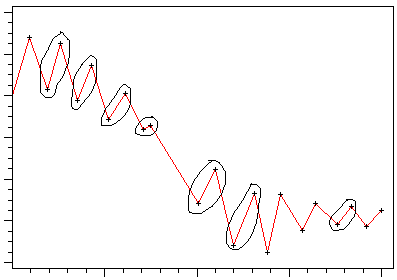
\includegraphics[width=0.84\textwidth]{Figures/LoaderRos9_pass0}
\caption{Rainflow analysis: Points defining full stress cycles detected
during the first traversal of the curve in Figure~\ref{fig:PVX}b).}
\label{fig:Rainflow1}
\end{figure}

\begin{figure}[t]
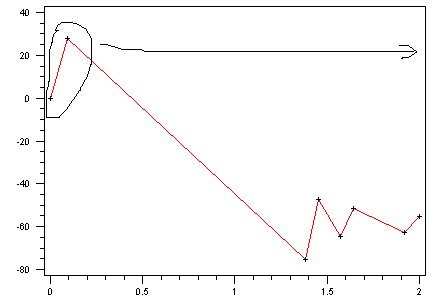
\includegraphics[width=0.5\textwidth]{Figures/LoaderRos9_pass1}
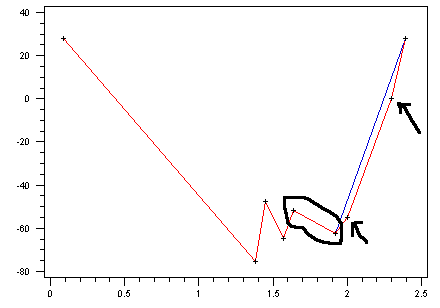
\includegraphics[width=0.5\textwidth]{Figures/LoaderRos9_pass2}
a) \hskip 0.5\textwidth b) \\[2mm]
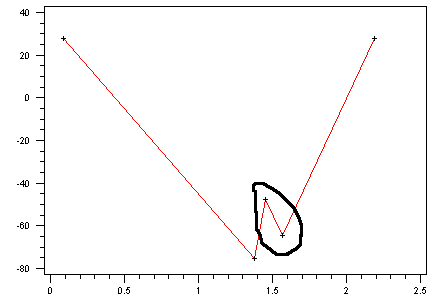
\includegraphics[width=0.5\textwidth]{Figures/LoaderRos9_pass3}
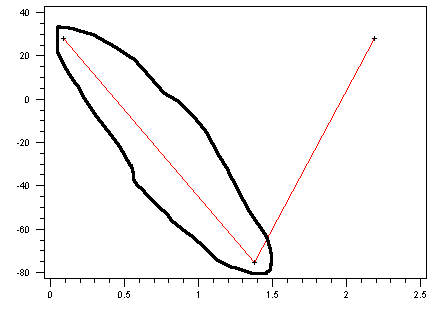
\includegraphics[width=0.5\textwidth]{Figures/LoaderRos9_pass4}
c) \hskip 0.5\textwidth d)
\caption{Subsequent steps of the rainflow analysis:
a) Inserting an additional max point making it the new start and end point.
b) Removing two `non-turning' points and the next full stress cycle.
c) Removing another full cycle in the next traversal.
d) Counting the final cycle.}
\label{fig:Rainflow2}
\end{figure}

Even when no more full cycles can be detected through the procedure outlined
above, there will normally still be some left-over points in the curve.
This is the situation already after the first traversal for the curve in
Figure~\ref{fig:Rainflow1}.
The remaining curve is then modified by duplicating the point with the largest
magnitude, and then shifting the added point and all preceding points to the
end of the curve, as illustrated by the arrow in Figure~\ref{fig:Rainflow2}a).
The modified curve then becomes as shown in Figure~\ref{fig:Rainflow2}b).
Here, the two points indicated by the arrows are not `turning points'.
They are therefore removed from the curve without counting a cycle, resulting
in the blue portion of the curve instead.
The traversal can now be repeated on the modified curve, until only three
points remain which then will count as the final cycle.
This process is depicted by the Figures~\ref{fig:Rainflow2}b-d),
where one cycle is detected in each traversal.

The rainflow counting outlined above can be performed in a similar manner for a
stress history and a strain history curve.
In Fedem it is only applied on stress history results.

\subsection{Damage and life calculation}

The rainflow analysis produces a list of stress ranges with magnitudes
$\bar{\sigma}_i$ representing the entire stress history in a given point for
the duration of the numerical simulation.
The accumulated damage in that point can now be computed using the S-N curve for
the material in question.

An S-N curve relates a stress range magnitude (S) to the number of repetitions
(N) of a cycle of that magnitude, a material point can sustain before failure.
S-N curves are typically derived from tests on samples of the material in
question, and may be found in various design codes for certain materials and
loading conditions.

For a given set of stress ranges, $\bar{\sigma}_i, i=1 \ldots k$, we read the
corresponding number of cycles before failure, $N_i$, from the specified
S-N, curve.
The accumulated damage is then computed as
%
\begin{equation}
C \;=\; \sum_{i=1}^k\frac{1}{N_i}
\end{equation}
%
and failure occurs when $C>=1.0$.
The estimated life in terms of number of repetitions of the simulated loading
event is then the reciprocal of this value, $1/C$.
If the simulated time span is denoted $T_s$, the estimated life at the
material point is therefore
%
\begin{equation}
\text{Life} \;=\; \frac{T_s}{C}
\end{equation}

\iftoggle{publicedition}{}{% The following is for the in-house edition only.
% SPDX-FileCopyrightText: 2023 SAP SE
%
% SPDX-License-Identifier: Apache-2.0
%
% This file is part of FEDEM - https://openfedem.org

%%%%%%%%%%%%%%%%%%%%%%%%%%%%%%%%%%%%%%%%%%%%%%%%%%%%%%%%%%%%%%%%%%%%%%%%%%%%%%%%
%
% FEDEM Theory Guide.
%
%%%%%%%%%%%%%%%%%%%%%%%%%%%%%%%%%%%%%%%%%%%%%%%%%%%%%%%%%%%%%%%%%%%%%%%%%%%%%%%%

\section{Eigenvalue results}

The general eigenvalue problem may be written
%
\begin{equation}
{\mf A}{\mf x} = \lambda{\mf B}{\mf x} \quad\text{or}\quad
({\mf A} -\lambda{\mf B}){\mf x} = {\mf 0}
\label{eqEIG:Def}
\end{equation}
%
where $\mf A$ and $\mf B$ need not necessarily be positive definite
or symmetrical.

\subsection{Undamped eigenvalue problem}

The second order differential equation governing free undamped vibration of the
discretized system can be written
%
\begin{equation}
{\mf M}\ddot{\mf v} + {\mf K}{\mf v} = {\mf 0}
\label{eqEIG:DiffUndamped}
\end{equation}
%
Assuming a solution of the form ${\mf v}(t) = {\mf v}_\lambda e^{\lambda_u t}$
gives
%
\begin{equation}
{\mf v}(t) \;=\; {\mf v}_{\lambda} e^{\lambda_u t}, \quad
\dot{\mf v}(t) \;=\; \lambda_u{\mf v}_{\lambda} e^{\lambda_u t}, \quad
\ddot{\mf v}(t) \;= \lambda_u^2{\mf v}_{\lambda} e^{\lambda_u t}
\label{eqEIG:AssumedSol}
\end{equation}
%
Substituting into \eqnref{eqEIG:DiffUndamped} gives
%
\begin{equation}
\left({\mf K} + \lambda_u^2 {\mf M}\right) {\mf v}_{\lambda} \;=\; {\mf 0}
\label{eqEIG:Undamp1}
\end{equation}
%
or
%
\begin{equation}
\left({\mf A} - \lambda{\mf B}\right){\mf x}_{\lambda} \;=\; {\mf 0}
\quad\text{where}\quad
\left\{\begin{array}{l}
{\mf A} \;=\; {\mf K} \\
{\mf B} \;=\; {\mf M} \\
\lambda \;=\; -\lambda_u^2 \quad\Rightarrow\quad \lambda_u = \sqrt{-\lambda}
\end{array}\right.
\label{eqEIG:Undamp2}
\end{equation}
%
When both $\mf A$ and $\mf B$ are positive definite, one will have positive
eigenvalues $\lambda$, and thus purely imaginary values for $\lambda_u$;
in other words, $\lambda_u = \text{i}\,\omega$.
In addition, because $\mf A$ and $\mf B$ are symmetrical, the eigenvectors
${\mf x}_{\lambda}$ are real.

The general solution of \eqsref{eqEIG:DiffUndamped}{eqEIG:Undamp2}
can then be written as
%
\begin{equation}
{\mf v}(t) \;=\; {\mf v}_{\lambda} e^{\text{i}\,\omega t} \;=\;
{\mf v}_{\lambda} \left(\cos\omega t + \text{i}\sin\omega t\right)
\label{eqEIG:UndampSolution}
\end{equation}
%
where the circle frequency $\omega$ is given by $\omega = \sqrt{\lambda}$.

\subsubsection{Animation of the eigenvectors}

The real and imaginary parts of the solution above are solutions of the original
homogeneous \eqnref{eqEIG:DiffUndamped}.
However, when animating the eigenvector, the real part of the solution of
\eqnref{eqEIG:UndampSolution} is displayed.
For example:
%
\begin{equation}
{\mf v}(t) \;=\; {\mf v}_{\lambda} \cos\omega t
\label{eqEIG:UndampAnimation}
\end{equation}



\subsection{Damped eigenvalue problem}

The second order differential equation governing free damped vibration of the
discretized system can be written
%
\begin{equation}
{\mf M}\ddot{\mf v} + {\mf C}\dot{\mf v}+ {\mf K}{\mf v} \;=\; {\mf 0}
\label{eqEIG:DiffDamped}
\end{equation}
%
Assuming a solution on the form ${\mf v}(t) = {\mf v}_{\lambda} e^{\lambda_d t}$
gives
%
\begin{equation}
{\mf v}(t) \;=\; {\mf v}_{\lambda} e^{\lambda_d t}, \quad
\dot{\mf v}(t) \;=\; \lambda_d{\mf v}_{\lambda} e^{\lambda_d t}, \quad
\ddot{\mf v}(t) \;=\; \lambda_d^2{\mf v}_{\lambda} e^{\lambda_d t}
\label{eqEIG:AssumedSol2}
\end{equation}
%
and substituting into \eqnref{eqEIG:DiffDamped} gives
%
\begin{equation}
\left({\mf K} + \lambda_d{\mf C} + \lambda_d^2{\mf M}\right){\mf v}_{\lambda}
\;=\; {\mf 0}
\label{eqEIG:Damp1}
\end{equation}
%
which cannot be cast directly into the form of \eqnref{eqEIG:Def}
unless the damping matrix $\mf C$ is given by Rayleigh damping:
${\mf C} = \alpha{\mf K} + \beta{\mf M}$
(see Section~\ref{sec:RayleighDamping}).

For a general damping matrix, the $n$-dimensional second order system of
\eqnref{eqEIG:DiffUndamped} can be cast into a first order system of dimension
$2n$ by introducing
%
\begin{equation}
{\mf u} \;= \left[\begin{array}{c} {\mf v} \\ \dot{\mf v} \end{array}\right]
\label{eqEIG:uDef}
\end{equation}
%
Equation~\eqref{eqEIG:uDef} allows a number of different ways of writing
\eqnref{eqEIG:DiffUndamped} as a first order equation; but to
preserve possible symmetry, the canonical form is chosen:
%
\begin{equation}
{\mf A u} - {\mf B}\dot{\mf u} \;=\; {\mf 0} \quad\text{where}\quad
\left\{\begin{array}{l}
{\mf A} \;= \left[\begin{array}{cc} {\mf K} & {\mf 0} \\ {\mf 0} & {\mf -M}
            \end{array}\right] \\[5mm]
{\mf B} \;= \left[\begin{array}{cc} {\mf -C} & {\mf -M} \\ {\mf -M} & {\mf 0}
            \end{array}\right]
\end{array}\right.
\label{eqEIG:Canonical}
\end{equation}
%
Assuming the solution on the form ${\mf u} = {\mf u}_\lambda e^{\lambda_d t}$
gives
%
\begin{equation}
{\mf u} \;=\; {\mf u}_\lambda e^{\lambda_d t}, \quad
\dot{\mf u} \;=\; \lambda_d{\mf u}_\lambda e^{\lambda_d t}
\label{eqEIG:AssumedSol3}
\end{equation}
%
and the first order eigenvalue problem has the familiar standard form
%
\begin{equation}
\left({\mf A} - \lambda_d{\mf B}\right){\mf u}_\lambda \;=\; {\mf 0}
\label{eqEIG:FirstOrderEig}
\end{equation}
%
In general, the solution of the damped eigenvalue problem above has
complex eigenvalues $\lambda_d$ and complex eigenvectors ${\mf u}_\lambda$:
%
\begin{equation}
\lambda_d \;=\; \mu + \text{i}\omega \qquad\text{and}\qquad
{\mf u}_\lambda \;=\; {\mf u}_{\Re} + \text{i}{\mf u}_{\Im} \;=
\left[\begin{array}{c}{\mf v}_{\Re} \\ \dot{\mf v}_{\Re} \end{array}\right] +
\text{i}\left[\begin{array}{c}{\mf v}_{\Im} \\ \dot{\mf v}_{\Im} \end{array}\right]
\label{eqEIG:EigSolDamp}
\end{equation}
%
The imaginary part $\omega$ signifies circle frequency, as in the undamped
problem; whereas the real part $\mu$ represents the damping of the eigenmode.
This value is (usually) a negative number, and tells at what rate the amplitude
of the free vibration will decrease.

A positive-values $\mu$ signifies an unstable system in which the amplitude
is increasing.
This can happen with axially loaded structures in which the axial load
is higher than the critical buckling load.
This gives a negative definite stiffness matrix and possible negative damping.

A negative-valued $\mu$ without an accompanying $\omega$, such as a real
eigenvalue, signifies a critically damped mode.

\subsubsection{Animation of complex eigenvectors}

Extracting the $n$ dimensional vector ${\mf v}_\lambda$ from the solution
\eqnref{eqEIG:AssumedSol3} and combining it with \eqnref{eqEIG:EigSolDamp} gives
%
\begin{equation}
\label{eqEIG:DampedSol}
\eqalign{{\mf v}(t)
\;=\; & e^{\lambda_d t}{\mf v}_\lambda
\;=\; e^{(\mu + \text{i}\omega)t}{\mf v}_\lambda
\;=\; e^{\mu t} e^{\text{i}\omega t} ({\mf v}_{\Re} + \text{i}{\mf v}_{\Im}) \cr
  =\; & e^{\mu t}(\cos\omega t + \text{i}\sin\omega t)
                 ({\mf v}_{\Re} + \text{i}{\mf v}_{\Im}) \cr
  =\; & e^{\mu t}\left[({\mf v}_{\Re}\cos\omega t - {\mf v}_{\Im}\sin\omega t) +
          \text{i}({\mf v}_{\Im}\cos\omega t +{\mf v}_{\Re}\sin\omega t)\right]}
\end{equation}
%
As in the undamped case, the real part of the solution is selected for animation
of the eigenvalue and eigenvector:
%
\begin{equation}
{\mf v}_{\Re}(t) \;=\;
e^{\mu t}({\mf v}_{\Re}\cos\omega t - {\mf v}_{\Im}\sin\omega t)
\end{equation}

\subsubsection{Diagonalizing the damped eigenvalue problem}

Having calculated a set of eigenvectors, ${\mf u}_{\lambda_i}$, the canonical
form~\eqref{eqEIG:Canonical}, the quadratic expression~\eqref{eqEIG:Damp1},
or the original differential \eqnref{eqEIG:DiffUndamped} can be diagonalized.
Of primary interest is diagonalizing the mass, stiffness
and damping matrices of \eqsref{eqEIG:Damp1}{eqEIG:DiffDamped}:
%
\begin{eqnarray}
m_i &=& \bar{\mf v}_{\lambda_i}^T {\mf M}{\mf v}_{\lambda_i} \nonumber \\
c_i &=& \bar{\mf v}_{\lambda_i}^T {\mf C}{\mf v}_{\lambda_i} \\
k_i &=& \bar{\mf v}_{\lambda_i}^T {\mf K}{\mf v}_{\lambda_i} \nonumber
\label{eq:modalMCK}
\end{eqnarray}
%
where $\bar{\mf v}_{\lambda_i}$ is the complex conjugate of ${\mf v}_{\lambda_i}$.
In other words:
%
\begin{equation}
{\mf v} \;=\; {\mf v}_{\Re} + \text{i}{\mf v}_{\Im}
\quad\text{and}\quad
\bar{\mf v} \;=\; {\mf v}_{\Re} - \text{i}{\mf v}_{\Im}
\end{equation}


\subsection{Calculating damping ratios}

Once the eigenvalues and eigenvectors have been calculated,
one can calculate damping ratios for the different eigenmodes.
For a single-DOF system with mass $m$, stiffness $k$ and damping $c$,
one has the undamped eigenvalue given by
%
\begin{equation}
\omega \;=\; \sqrt{\frac{k}{m}}
\end{equation}

For a system with damping one can show that no true vibration will occur when
the damping $c$ is sufficiently high; called critical damping $c_\textit{cr}$.
In this case the dynamic motion will be an asymptotic motion to the static
equilibrium position.
The critical damping is given by
%
\begin{equation}
c_\textit{cr} \;=\; 2 m \omega %= 2 m \sqrt{\frac{k}{m}} = 2 \sqrt{k m}
\end{equation}

The critical damping is a convenient reference point for describing
the amount of damping in a system.
This is done by defining the damping ratio
%
\begin{equation}
\xi \;=\; \frac{c}{c_\textit{cr}} = \frac{c}{2 m \omega}
\end{equation}
%
This is often given in percent (\%) of the critical damping.

\subsubsection{Based on damped eigenvalue problem}

The eigenvectors ${\mf v}_{\lambda_i}$ for each eigenmode $i$ of the damped
system will diagonalize the mass, stiffness, and damping matrix
as given by \eqnref{eq:modalMCK}.
This gives the damping ratio for eigenmode $i$ as
%
\begin{equation}
\xi_i \;=\; \frac{c_i}{c_{\textit{cr}_i}} = \frac{c_i}{2 \sqrt{k_i m_i}}
\end{equation}

\subsubsection{Based on undamped eigenvalue problem}

The eigenvectors ${\mf v}_{\lambda_i}$ for each eigenmode $i$ of the undamped
system will diagonalize the mass matrix, i.e. create the modal mass
%
\begin{equation}
m_i \;=\; {\mf v}_{\lambda_i}^T {\mf C}{\mf v}_{\lambda_i}
\label{eq:modalMass}
\end{equation}

An approximate damping coefficient can be calculated based on the
same eigenvector
%
\begin{equation}
c_i \;\approx\; {\mf v}_{\lambda_i}^T {\mf C}{\mf v}_{\lambda_i}
\label{eq:approxDampingCoeff}
\end{equation}
%
which gives an approximate damping ratio
%
\begin{equation}
\xi_i \;\approx\; \frac{c_i}{2 m_i \omega_i} = \frac{c_i}{2\sqrt{k_i m_i}}
\end{equation}

Note that if the damping matrix constitutes Rayleigh damping, see
Section~\ref{sec:RayleighDamping}, the damping ratios calculated above are exact.
For damping ratios $\ll 1$ the approximation is very good
also for a more general damping matrix.


\subsection{Using shift when solving the eigenvalue problem}

To improve the convergence of the iterations, or to find eigenvalues in the
neighborhood of a particular value, a \textit{shift} can be applied to the
initial eigenvalue problem.
The eigenvalue problem $({\mf K} - \lambda {\mf M}){\mf v} = {\mf 0}$ may be
written as the equivalent expression
%
\begin{equation}
\left( \hat{\mf K} - \hat{\lambda}{\mf M} \right) {\mf v} \;=\; {\mf 0}
\quad\text{where}\quad
\hat{\mf K} \;=\; {\mf K} - \mu{\mf M}
\label{eqK25:21}
\end{equation}
%
and $\mu$ is the shift value.
The modified eigenvalues $\hat{\lambda}_i$ are given by the relation
%
\begin{equation}
\hat{\lambda}_i \;=\; \lambda_{i} - \mu
\end{equation}
%
where $\lambda_i$ represents the eigenvalues and  the eigenvectors are the same
as those in the original eigenvalue problem.

Matrix $\hat{\mf K}$ must be invertible.
If, for instance, the original $\mf K$ is not positive definite, as is the case
with a free structure, a negative shift can be applied that makes the matrix
$\hat{\mf K}$ positive definite.
This makes it possible to find the zero frequency (rigid body) modes of a free
system, as well as the other lowest eigenvalues and eigenvectors.

The iteration procedure for eigenvalue solvers, such as Lanczos and sub-space
iterations, converges toward a set of eigenvectors that have corresponding
eigenvalues closest to $\mu$, which are a set of eigenvalues with
$\hat{\lambda}_i=\lambda_i-\mu$ and the smallest absolute value.
This procedure can be used to add desired generalized modes around a particular
frequency for the CMS-reduction of Chapter~\ref{chap:CMS}.

} % End in-house edition only
% SPDX-FileCopyrightText: 2023 SAP SE
%
% SPDX-License-Identifier: Apache-2.0
%
% This file is part of FEDEM - https://openfedem.org

%%%%%%%%%%%%%%%%%%%%%%%%%%%%%%%%%%%%%%%%%%%%%%%%%%%%%%%%%%%%%%%%%%%%%%%%%%%%%%%%
%
% FEDEM Theory Guide.
%
%%%%%%%%%%%%%%%%%%%%%%%%%%%%%%%%%%%%%%%%%%%%%%%%%%%%%%%%%%%%%%%%%%%%%%%%%%%%%%%%

\section{Energy calculations}

Energy calculations are described by the following terms:

\begin{namelist}{$U_{sum}$}

\item[$U_\varepsilon$]
Strain energy,  computed for all links (superelements), springs, 
and the system (the system is the sum of all mechanisms)

\item[$U_{k}$]
Kinetic energy,  computed for all links, 
discrete masses, rotational inertias, and the system

\item[$U_{p}$]
Potential energy,  computed for all links, 
discrete masses, and the system

\item[$U_{i}$]
Input energy,  computed for all external forces, 
springs (contribution from non-constant, stress-free length), and the system

\item[$U_{d}$]
Energy loss,  computed for all links (structural 
damping), axial dampers, joint dampers, joint friction, and the system

\item[$U_{e}$]
External energy, computed for all external ``elements'', such as tires, that are using
$3^\text{rd}$ party software modules. The energy can be one of (or a mix of) strain,
damping, and other energy terms.

\item[$U_{sum}$]
Energy check-sum, computed for the system
\end{namelist}

\noindent
All these terms are can be plotted as functions of time or other 
variables.

\subsection{Strain energy}

The total strain energy for the system is computed as a sum of all the 
element strain energies and spring strain energies.

\subsubsection{Link strain energy}

The strain energy for one link with linearly elastic 
material is given by


\begin{equation}
U_{\varepsilon } = \frac{{1}}{{2}}{\mf v}_{d}^{T} {\mf K}{\mf v}_{d}
\label{eqEC:81}
\end{equation}

\noindent
where ${\mf v}_{d}$ is the deformational displacement of the 
element, and ${\mf K}$ is the element stiffness matrix. The strain 
energy is thus computed on a total form at each converged time-step; in other words, no 
storage of previous strain energy is necessary.

\subsubsection{Spring strain energy}

Even the nonlinear springs have hyper-elastic behavior, and the strain 
energy is computed totally at each converged time-step.
%
\begin{eqnarray}
\mbox{Linear springs :\ \ } && U_{\varepsilon} = \frac{{1}}{{2}}k_{s} u^{2} \\
\mbox{Nonlinear springs:\ \ } && U_{\varepsilon } = \int_{0}^{u} f_{s} \left( 
{\hat u} \right) d{\hat u}  \nonumber
\label{eqEC:82}
\end{eqnarray}
%
\noindent
As the expression for the hyper-elastic, nonlinear spring energy also 
includes the linear spring element, it is used for all spring elements, linear and nonlinear,
and for axial and joint springs. Incremental calculations of the spring strain energy are not
necessary as long as only hyper-elastic nonlinear springs are included in the model.

\subsection{Kinetic energy}

System kinetic energy consists of the contributions from all the links, all 
the lumped masses, and all the discrete rotational inertias.

\subsubsection{Link kinetic energy}

The link kinetic energy is calculated from the superelement 
mass matrix, ${\mf M}$ and the superelement velocity vector, 
$\dot{\mf v}$, as:
%
\begin{equation}
U_{k} = \frac{{1}}{{2}} \dot{\mf v}^{T}{\mf M}
\dot{\mf v} .
\label{eqEC:84}
\end{equation}
%
\noindent
In other words, it is also computed on a total form for each time-step.

\subsubsection{Kinetic energy from discrete masses and inertias}

Discrete masses and rotational inertias contribute to the kinetic energy as:
%
\begin{equation}
U_{k} = \frac{{1}}{{2}}m \dot{\mf u}^{T} 
\dot{\mf u} + \frac{{1}}{{2}}{\tf{\omega}}^{T}{\mf I}_{\omega} \tf\omega ,
\label{eqEC:85}
\end{equation}
%
\noindent
where ${m}$ is the lumped mass and ${\mf I}_\omega $ is the 
rotational inertia matrix for the lumped mass.

\subsection{Potential energy}

As is the case with the kinetic energy, the system's potential energy is the sum off all 
the contributions from the links and the discrete masses. However, the 
discrete rotational inertias do not contribute to the potential energy.

\subsubsection{Link potential energy}

Computation of the potential energy should reflect the changes in potential 
energy rather than the potential energy in relation to the coordinate system 
used for modeling. Choosing a coordinate system which gives large potential energies may hide
other energy contributions. 
By subtracting the potential energy of the masses in their 
initial position ${C_0}$ from the potential energy at the present position ${C_n}$, the initial

potential energy of all masses, superelement masses, and lumped masses is zero.
%
\begin{equation}
U_{p} = m{\mf g}^{T}\left( {\mf x}_{C_n} - {\mf x}_{C_0}  \right)
\label{eqEC:86}
\end{equation}
%
\noindent
Calculations of the potential energy of the links use the displacements of 
the link centroid. This calculation neglects the relative displacement of 
the centroid due to internal deformations of the superelements; however 
this is justified by assuming small deformations. The 
calculation of the potential energy is performed entirely without 
storing energies from previous steps.

\subsection{Input energy}

Input energy to the system consists of contributions from external forces 
and springs that have non-constant, stress-free length.

\subsubsection{Input energy from external forces}

Since the external forces are non-conservative (i.e., can have a time variation 
and co-rotational behavior), the input energy from the external forces must 
be computed in an incremental manner from one time-step to the next:
%
\begin{equation}
 U_{i} = \int_{0}^{t} {{\mf F}^T\!\left( { {\hat t} }\right) \dot{\mf u} \,d{\hat t} 
\approx \sum_{k = 1}^{n} {\overline {{\mf F}}_{k}^{T}\Delta {\mf u}_{k} } } 
 \mbox{\ \ \ \ where\ \ \ \ }
\overline{{\mf F}}_{k}  = \frac{{1}}{{2}}\left( {\mf F}_{k - 1} + {\mf F}_{k}  \right)
\label{eqEC:87}
\end{equation}
%
Subscript $k$ is the time-step index. The summation expression 
above represents a trapezoidal integration scheme.

\subsubsection{Input energy from springs}

The stress-free lengths of the springs (both axial springs and joint springs) 
are subject to possible change. When the spring is 
stressed, this represents an input energy contribution. This input energy 
must be computed incrementally for all the springs:
%
\begin{equation}
 U_{i} = 
\int_{0}^{t} f_{s}({\hat t}) l_{0} \:d{\hat t} \approx \sum_{k = 1}^{n} 
\overline{f}_{s_{k}}  \Delta l_{0}  
 \mbox{\ \ \ \ where\ \ \ \ }
\overline {f}_{s_{k}} = 
\frac{{1}}{{2}}(f_{s_{k-1}} + f_{s_{k}})
\label{eqEC:88}
\end{equation}

\subsection{Energy loss}

Total energy loss consists of the contributions from structural damping 
in the links and discrete dampers (both axial dampers and joint dampers), and 
energy loss from joint friction.

\subsubsection{Energy loss from link structural damping}

The structural damping of the links is composed of mass and stiffness 
proportional damping  (${\mf C} = \alpha_{1}{\mf M}+\alpha_{2}{\mf K}$),
which is used in the following damping energy expression for a link
%
\begin{equation}
U_{d} = \int_{0}^{t} { \dot{\mf v}^{T}{\mf C}
\dot{\mf v} d {\hat t}} 
\approx \sum_{k = 1}^{n} h\alpha _{1}  \bar{\dot{{\mf v}}}_k^T{\mf M}\bar{\dot{{\mf v}}}_k 
+ \sum_{k = 1}^{n} h\alpha _{2}  {\dot{\mf v}{}_d}_{k}^T {\mf K}  {\dot{\mf v}{}_d}_k
\label{eqEC:89}
\end{equation}
%
\noindent
where 
$ \bar{\dot{{\mf v}}}_{k}^{T} = \frac{{1}}{{2}}\left(\dot{\mf v}_{k-1} 
                                           + \dot{\mf v}_{k}  \right)$,
and 
$ {\dot{\mf v}{}_d}_k = \frac{{1}}{{h}}\left( {{\mf v}_d}_{k} 
                                            - {{\mf v}_d}_{k-1} \right)$,
and 
${h}$ represent the time-step size.
%
Note that the deformational velocities, $ {\dot {\mf v}_d} $, are used
when computing the stiffness proportional damping 
energy. This is important to avoid false damping energies from 
rigid-body velocities when using large time-steps.

\subsubsection{Energy loss from discrete dampers}

Energy loss from discrete dampers (axial dampers and joint dampers) is 
computed as
%
\begin{equation}
U_{d} = \int_{0}^{t} f_{d}  {\dot u} \:dt \approx 
\sum_{k = 1}^{n} {\overline{f}{}_d}_k  \Delta u  
\label{eqEC:810}
\end{equation}
%
\noindent
where 
${\overline{f}{}_d}_k = \frac{1}{2}\left( {f_d}_{k-1} + 
{f_d}_k \right)$

\subsubsection{Energy loss from friction}

Friction energy loss is computationally analogous to the damping loss
%
\begin{equation}
U_{d} = \int_{0}^{t} f_{f}\:dt \approx \sum_{k=1}^{n} {\overline{f}{}_f}_k  \Delta u_{k}   
\end{equation}
%
\noindent
where 
${\overline{f}{}_f}_k = \frac{1}{2}\left( {f_f}_{k-1} + 
{f_f}_k \right)$ 

\subsection{External energy}

External energy from 3rd party components such as tires is calculated
is calculated through the incremental work performed at the component interface
from one time-step to the next:
%
\begin{equation}
 U_{e} = \int_{0}^{t} {{\mf F}^T\!\left( { {\hat t} }\right) \dot{\mf u} \:d{\hat t} 
\approx \sum_{k = 1}^{n} {\overline {{\mf F}}_{k}^{T}\Delta {\mf u}_{k} } } 
 \mbox{\ \ \ \ where\ \ \ \ }
\overline{{\mf F}}_{k}  = \frac{{1}}{{2}}\left( {\mf F}_{k - 1} + {\mf F}_{k}  \right)
\label{eqEC:83}
\end{equation}
%
Subscript $k$ is the time-step index. The summation expression 
above represents a trapezoidal integration scheme. The forces $\mf F$ from the
component can have contribution from both stiffness and damping forces, 
and the energy contribution is thus a mixed energy. 


\subsection{Energy check-sum}

An energy check-sum is computed for the system to verify that the 
system energy is preserved:
%
\begin{equation}
U_{\text{sum}} = {U_p}_{\text{system}}  + {U_k}_{\text{system}}  
               + {U_\varepsilon}_{\text{system}}  
               + {U_d}_{\text{system}} - {U_i}_{\text{system}} - {U_e}_{\text{system}}
\label{eqEC:811}
\end{equation}
%
\noindent
The check-sum should remain constant during time integration.

